\section{Versuchsaufbau}
In Abbildung \ref{fig:aufbau} ist eine Schemazeichnung des aufgebauten Experiments zu sehen. Das Experiment beinhaltet eine optische Pinzette und ein Mikroskop zur Beobachtung der behandelten Probe.
\begin{figure}[H]
  \centering
  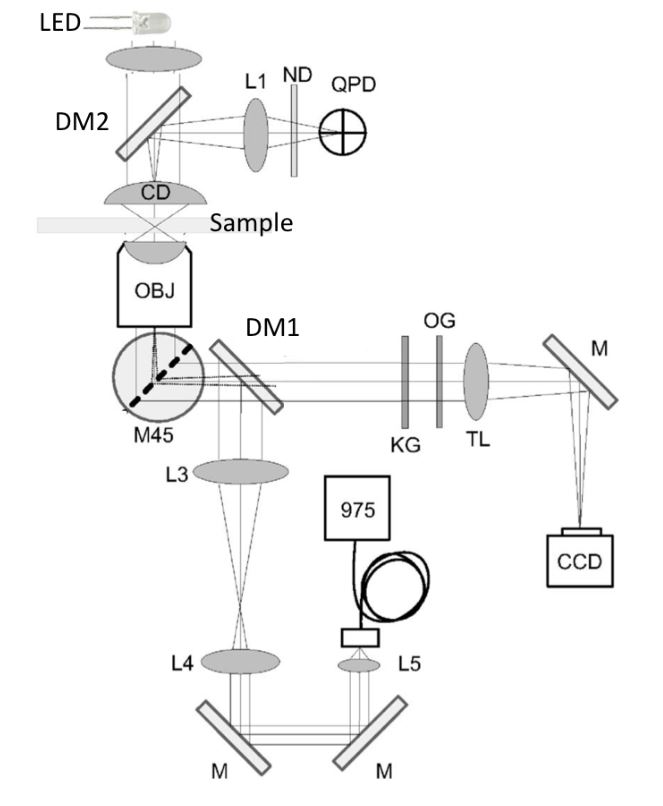
\includegraphics[width=0.5\textwidth]{plots/aufbau.jpg}
  \caption{Schemazeichnung des Aufbaus der optischen Pinzette mit zusätzlichem Lichtmikroskop. \cite{anleitung}}
  \label{fig:aufbau}
\end{figure}
Das Mikroskop besteht aus einer Weisslicht-LED, deren Licht über eine Linse und einen dichroistischen Spiegel (DM2) in das Mikroskopobjektiv fokussiert wird. Über einen weiteren dichroistischen Spiegel (DM1) wird das Licht anschließend zu einer CCD-Kamera geleitet, die an einen PC angeschlossen ist.\\
Die optische Pinzette besteht aus einem $975 \si{\nano\meter}$ Laser, der über eine Glasfaser in die Apparatur eingekoppelt wird. Mithilfe weiterer Spiegel, des dichroistischen Spiegels DM1 und eines Teleskops wird das Licht anschließend durch ein weiteres Objektiv mit hoher numerischer Appertur auf die Probe fokussiert. Anschließend wird der Laserstrahl mithilfe einer Viersegment-Photodiode detektiert.
Die dichroistischen Spiegel erlauben es Mikroskop- und Laserlicht auf der Probe zu überlagern und anschließend wieder zu trennen, sodass keine Störeinflüsse in der CCD-Kamera bzw. in der Viersegment-Photodiode auftreten. Die vier Segmente der Photodiode sind so miteinander verschaltet, dass das Ausgangssignal bei Position des Laserspots im Zentrum der Diode gleich Null ist. Je nach Auslenkung aus dieser Ruhelage ergibt sich ein positives oder negatives Ausgangssignal in $x$- und $y$- Richtung. Um die Numerische Appertur der Apparatur zu erhöhen wird ein Tropfen Immersionsöl auf das sich unter der Probe befindende Objektiv gegeben. \\
Die Position der Probe im Aufbau ist sowohl manuell über einen mit Mikrometerschrauben versehenen Probentisch, als auch elektronisch über Piezoelemente in allen drei Raumrichtungen einstellbar. Mithilfe der \textit{strain-gauge} Methode kann ausserdem die Ausdehnung der Piezokristalle (und damit die Position der Probe) digital kontrolliert werden.

\section{Durchführung}
\subsection{Messung der Fallensteifigkeit über Zeitserien}
Um die Fallensteifigkeit über das Äquipartitionstheorem zu vermessen, werden zeitaufgelößte Messungen der Bewegung einer Glasspähre aufgenommen. Dabei werden Messungen eines Teilchens in der optischen Falle ohne Krafteinwirkung und mit Krafteinwirkung in $x$- bzw. $y$-Richtung vorgenommen. Die durchschnittlich $2 \si{\micro\meter}$ großen Glassphären werden dafür in entionisiertem destilliertem Wasser untersucht. Die Messungen werden für Laserleistungen zwischen $70\si{\milli\watt}$ und $470\si{\milli\watt}$ durchgeführt. Zusätzlich wird das Bild der CCD-Kamera aufgenommen. Anschließend werden alle Messungen für Polystyrenkugeln mit einem ungefähren Durchmesser von $0.6\si{\micro\meter}$ durchgeführt.\\
Für die Messungen mit Krafteinwirkung vereinfacht sich die Differentialgleichung der Bewegung des Teilchens zu
\begin{equation}
  \beta \dot x = kx \, ,
\end{equation}
da die Brownsche Bewegung des eingefangenen Teilchens vernachlässigt werden kann.

\subsection{Kalibration der Spannung der Viersegment-Photodiode}
Um an der Photodiode anliegende Ausgangssignal in eine Position umwandeln zu können wird der Spannungs-Positions-Konversionsfaktor der Diode bestimmt. Dafür werden einer Probe aus Glasspähren in destilliertem Wasser NaCl-Ionen beigefügt, um die Debeye-Abschirmung der Sphären zu reduzieren. Die Sphären sind jetzt in der Lage fest an der Probenbehälterwand anzuhaften. Für die Positionskalibrierung wird nun mithilfe der Piezosteuerung ein Leistungsprofil an der Photodiode aufgenommen, welches von der $x$- bzw. $y$- Position des Laserspots auf der Probe abhängt.

\subsection{Untersuchung der Zwiebelzellen}
Zur Untersuchung der Bewegung von Vesikeln in Aktin-Filamenten wird eine Monolage einer Zwiebel in destilliertem, mit NaCl-Ionen versetztem Wasser auf einem Objektträger präpariert. Anschließend wird ein unbeschädigter Bereich der Zwiebel unter dem Mikroskop ausgewählt. Zunächst werden Videos der Bewegung der Vesikeln in den Kanälen und der Manipulation der Vesikeln mit der optischen Pinzette aufgenommen. Anschließend wird die optische Pinzette bei einer Leistung von $70 \si{\milli\watt}$ auf einen Aktin-Myosin Kanal ausgerichtet um die Geschwindigkeit der Vesikeln bei Bewegung durch das Filament zu bestimmen. Die Leistung wird danach schrittweise erhöht bis die Vesikel die optische Falle nicht mehr Verlassen können.\\
Um die Reißfestigkeit der Filamente zu bestimmen wird ein Teilchen bei ausreichender Leistung eingefangen und anschließend der Objektträger bewegt, sodass das Teilchen aus dem Filament ausbricht oder das Filament zerreist.\\
Bei den Messungen an der Zwiebel ist zu beachten, dass die Lebensdauer der Zwiebelzellen auf 30 bis 60 Minuten begrenzt ist.\\
